\documentclass[12pt,a4paper]{article}

\usepackage[a4paper,text={16.5cm,25.2cm},centering]{geometry}
\usepackage{lmodern}
\usepackage{amssymb,amsmath}
\usepackage{bm}
\usepackage{graphicx}
\usepackage{microtype}
\usepackage{hyperref}
\setlength{\parindent}{0pt}
\setlength{\parskip}{1.2ex}

\hypersetup
       {   pdfauthor = { Daniele Zago and Giovanna Capizzi },
           pdftitle={ Supplemental material },
           colorlinks=TRUE,
           linkcolor=black,
           citecolor=blue,
           urlcolor=blue
       }

\title{ Supplemental material }

\author{ Daniele Zago and Giovanna Capizzi }

\date{ 2022-09-28 }

\usepackage{upquote}
\usepackage{listings}
\usepackage{xcolor}
\lstset{
    basicstyle=\ttfamily\footnotesize,
    upquote=true,
    breaklines=true,
    breakindent=0pt,
    keepspaces=true,
    showspaces=false,
    columns=fullflexible,
    showtabs=false,
    showstringspaces=false,
    escapeinside={(*@}{@*)},
    extendedchars=true,
}
\newcommand{\HLJLt}[1]{#1}
\newcommand{\HLJLw}[1]{#1}
\newcommand{\HLJLe}[1]{#1}
\newcommand{\HLJLeB}[1]{#1}
\newcommand{\HLJLo}[1]{#1}
\newcommand{\HLJLk}[1]{\textcolor[RGB]{148,91,176}{\textbf{#1}}}
\newcommand{\HLJLkc}[1]{\textcolor[RGB]{59,151,46}{\textit{#1}}}
\newcommand{\HLJLkd}[1]{\textcolor[RGB]{214,102,97}{\textit{#1}}}
\newcommand{\HLJLkn}[1]{\textcolor[RGB]{148,91,176}{\textbf{#1}}}
\newcommand{\HLJLkp}[1]{\textcolor[RGB]{148,91,176}{\textbf{#1}}}
\newcommand{\HLJLkr}[1]{\textcolor[RGB]{148,91,176}{\textbf{#1}}}
\newcommand{\HLJLkt}[1]{\textcolor[RGB]{148,91,176}{\textbf{#1}}}
\newcommand{\HLJLn}[1]{#1}
\newcommand{\HLJLna}[1]{#1}
\newcommand{\HLJLnb}[1]{#1}
\newcommand{\HLJLnbp}[1]{#1}
\newcommand{\HLJLnc}[1]{#1}
\newcommand{\HLJLncB}[1]{#1}
\newcommand{\HLJLnd}[1]{\textcolor[RGB]{214,102,97}{#1}}
\newcommand{\HLJLne}[1]{#1}
\newcommand{\HLJLneB}[1]{#1}
\newcommand{\HLJLnf}[1]{\textcolor[RGB]{66,102,213}{#1}}
\newcommand{\HLJLnfm}[1]{\textcolor[RGB]{66,102,213}{#1}}
\newcommand{\HLJLnp}[1]{#1}
\newcommand{\HLJLnl}[1]{#1}
\newcommand{\HLJLnn}[1]{#1}
\newcommand{\HLJLno}[1]{#1}
\newcommand{\HLJLnt}[1]{#1}
\newcommand{\HLJLnv}[1]{#1}
\newcommand{\HLJLnvc}[1]{#1}
\newcommand{\HLJLnvg}[1]{#1}
\newcommand{\HLJLnvi}[1]{#1}
\newcommand{\HLJLnvm}[1]{#1}
\newcommand{\HLJLl}[1]{#1}
\newcommand{\HLJLld}[1]{\textcolor[RGB]{148,91,176}{\textit{#1}}}
\newcommand{\HLJLs}[1]{\textcolor[RGB]{201,61,57}{#1}}
\newcommand{\HLJLsa}[1]{\textcolor[RGB]{201,61,57}{#1}}
\newcommand{\HLJLsb}[1]{\textcolor[RGB]{201,61,57}{#1}}
\newcommand{\HLJLsc}[1]{\textcolor[RGB]{201,61,57}{#1}}
\newcommand{\HLJLsd}[1]{\textcolor[RGB]{201,61,57}{#1}}
\newcommand{\HLJLsdB}[1]{\textcolor[RGB]{201,61,57}{#1}}
\newcommand{\HLJLsdC}[1]{\textcolor[RGB]{201,61,57}{#1}}
\newcommand{\HLJLse}[1]{\textcolor[RGB]{59,151,46}{#1}}
\newcommand{\HLJLsh}[1]{\textcolor[RGB]{201,61,57}{#1}}
\newcommand{\HLJLsi}[1]{#1}
\newcommand{\HLJLso}[1]{\textcolor[RGB]{201,61,57}{#1}}
\newcommand{\HLJLsr}[1]{\textcolor[RGB]{201,61,57}{#1}}
\newcommand{\HLJLss}[1]{\textcolor[RGB]{201,61,57}{#1}}
\newcommand{\HLJLssB}[1]{\textcolor[RGB]{201,61,57}{#1}}
\newcommand{\HLJLnB}[1]{\textcolor[RGB]{59,151,46}{#1}}
\newcommand{\HLJLnbB}[1]{\textcolor[RGB]{59,151,46}{#1}}
\newcommand{\HLJLnfB}[1]{\textcolor[RGB]{59,151,46}{#1}}
\newcommand{\HLJLnh}[1]{\textcolor[RGB]{59,151,46}{#1}}
\newcommand{\HLJLni}[1]{\textcolor[RGB]{59,151,46}{#1}}
\newcommand{\HLJLnil}[1]{\textcolor[RGB]{59,151,46}{#1}}
\newcommand{\HLJLnoB}[1]{\textcolor[RGB]{59,151,46}{#1}}
\newcommand{\HLJLoB}[1]{\textcolor[RGB]{102,102,102}{\textbf{#1}}}
\newcommand{\HLJLow}[1]{\textcolor[RGB]{102,102,102}{\textbf{#1}}}
\newcommand{\HLJLp}[1]{#1}
\newcommand{\HLJLc}[1]{\textcolor[RGB]{153,153,119}{\textit{#1}}}
\newcommand{\HLJLch}[1]{\textcolor[RGB]{153,153,119}{\textit{#1}}}
\newcommand{\HLJLcm}[1]{\textcolor[RGB]{153,153,119}{\textit{#1}}}
\newcommand{\HLJLcp}[1]{\textcolor[RGB]{153,153,119}{\textit{#1}}}
\newcommand{\HLJLcpB}[1]{\textcolor[RGB]{153,153,119}{\textit{#1}}}
\newcommand{\HLJLcs}[1]{\textcolor[RGB]{153,153,119}{\textit{#1}}}
\newcommand{\HLJLcsB}[1]{\textcolor[RGB]{153,153,119}{\textit{#1}}}
\newcommand{\HLJLg}[1]{#1}
\newcommand{\HLJLgd}[1]{#1}
\newcommand{\HLJLge}[1]{#1}
\newcommand{\HLJLgeB}[1]{#1}
\newcommand{\HLJLgh}[1]{#1}
\newcommand{\HLJLgi}[1]{#1}
\newcommand{\HLJLgo}[1]{#1}
\newcommand{\HLJLgp}[1]{#1}
\newcommand{\HLJLgs}[1]{#1}
\newcommand{\HLJLgsB}[1]{#1}
\newcommand{\HLJLgt}[1]{#1}


\begin{document}

\maketitle

Here, we implement the code that reproduces the analysis on the ICU dataset in Section 5 of the paper.

First, we load the necessary packages and the environment variables that are provided in the source code.



\begin{lstlisting}
(*@\HLJLk{using}@*) (*@\HLJLn{DrWatson}@*)
(*@\HLJLcs{{\#}@quickactivate}@*) (*@\HLJLcs{"{}CautiousLearning"{}}@*)
(*@\HLJLnf{quickactivate}@*)(*@\HLJLp{(}@*)(*@\HLJLs{"{}}@*)(*@\HLJLsi{{\$}}@*)(*@\HLJLp{(}@*)(*@\HLJLnf{homedir}@*)(*@\HLJLp{())}@*)(*@\HLJLs{/Documents/git/SPC/CautiousLearning"{}}@*)(*@\HLJLp{)}@*)

(*@\HLJLk{using}@*) (*@\HLJLn{Distributions}@*)(*@\HLJLp{,}@*) (*@\HLJLn{Random}@*)
(*@\HLJLk{using}@*) (*@\HLJLn{Parameters}@*)
(*@\HLJLk{using}@*) (*@\HLJLn{SharedArrays}@*)
(*@\HLJLk{using}@*) (*@\HLJLn{DataFrames}@*)(*@\HLJLp{,}@*) (*@\HLJLn{CSV}@*)(*@\HLJLp{,}@*) (*@\HLJLn{Dates}@*)
(*@\HLJLk{using}@*) (*@\HLJLn{Plots}@*)(*@\HLJLp{,}@*) (*@\HLJLn{StatsBase}@*)(*@\HLJLp{,}@*) (*@\HLJLn{StatsPlots}@*)(*@\HLJLp{,}@*) (*@\HLJLn{LaTeXStrings}@*)(*@\HLJLp{,}@*) (*@\HLJLn{RCall}@*)
(*@\HLJLk{using}@*) (*@\HLJLn{StatisticalProcessControl}@*)

(*@\HLJLnf{include}@*)(*@\HLJLp{(}@*)(*@\HLJLnf{srcdir}@*)(*@\HLJLp{(}@*)(*@\HLJLs{"{}generate{\_}data.jl"{}}@*)(*@\HLJLp{))}@*)
(*@\HLJLnf{include}@*)(*@\HLJLp{(}@*)(*@\HLJLnf{srcdir}@*)(*@\HLJLp{(}@*)(*@\HLJLs{"{}update{\_}parameter.jl"{}}@*)(*@\HLJLp{))}@*)
(*@\HLJLnf{include}@*)(*@\HLJLp{(}@*)(*@\HLJLnf{srcdir}@*)(*@\HLJLp{(}@*)(*@\HLJLs{"{}simulate{\_}runs.jl"{}}@*)(*@\HLJLp{))}@*)
\end{lstlisting}

\begin{lstlisting}
Error: LoadError: UndefVarError: SimulationSettings not defined
in expression starting at /home/dede/Documents/git/SPC/CautiousLearning/src
/simulate(*@{{\_}}@*)runs.jl:206
\end{lstlisting}


First, we load the dataset which is located in the \texttt{data/ICUadmissions} folder, relative to the main directory of the project. We consider the data concerning the New York City area in 2020.


\begin{lstlisting}
(*@\HLJLn{fold}@*) (*@\HLJLoB{=}@*) (*@\HLJLs{"{}ICUadmissions"{}}@*)
(*@\HLJLn{dat}@*) (*@\HLJLoB{=}@*) (*@\HLJLnf{DataFrame}@*)(*@\HLJLp{(}@*)(*@\HLJLn{CSV}@*)(*@\HLJLoB{.}@*)(*@\HLJLnf{File}@*)(*@\HLJLp{(}@*)(*@\HLJLnf{datadir}@*)(*@\HLJLp{(}@*)(*@\HLJLn{fold}@*)(*@\HLJLp{,}@*) (*@\HLJLs{"{}New{\_}York{\_}Forward{\_}COVID-19{\_}Daily{\_}Hospitalization{\_}Summary{\_}by{\_}Region.csv"{}}@*)(*@\HLJLp{)))}@*)
(*@\HLJLn{nydat}@*) (*@\HLJLoB{=}@*) (*@\HLJLnf{filter}@*)(*@\HLJLp{(}@*)(*@\HLJLn{row}@*) (*@\HLJLoB{->}@*) (*@\HLJLn{row}@*)(*@\HLJLoB{.}@*)(*@\HLJLn{Region}@*) (*@\HLJLoB{==}@*) (*@\HLJLs{"{}NEW}@*) (*@\HLJLs{YORK}@*) (*@\HLJLs{CITY"{}}@*)(*@\HLJLp{,}@*) (*@\HLJLn{dat}@*)(*@\HLJLp{)}@*)
(*@\HLJLn{nydat}@*)(*@\HLJLoB{.}@*)(*@\HLJLn{date}@*) (*@\HLJLoB{.=}@*) (*@\HLJLn{Date}@*)(*@\HLJLoB{.}@*)(*@\HLJLp{(}@*)(*@\HLJLn{nydat}@*)(*@\HLJLp{[}@*)(*@\HLJLoB{:}@*)(*@\HLJLp{,}@*) (*@\HLJLni{1}@*)(*@\HLJLp{],}@*) (*@\HLJLso{dateformat"{}mm/dd/yyyy"{}}@*)(*@\HLJLp{)}@*)
(*@\HLJLn{nydat}@*) (*@\HLJLoB{=}@*) (*@\HLJLnf{filter}@*)(*@\HLJLp{(}@*)(*@\HLJLn{row}@*) (*@\HLJLoB{->}@*) (*@\HLJLnf{year}@*)(*@\HLJLp{(}@*)(*@\HLJLn{row}@*)(*@\HLJLoB{.}@*)(*@\HLJLn{date}@*)(*@\HLJLp{)}@*) (*@\HLJLoB{==}@*) (*@\HLJLni{2020}@*)(*@\HLJLp{,}@*) (*@\HLJLn{nydat}@*)(*@\HLJLp{);}@*)
\end{lstlisting}


We obtain the daily ICU counts along with the corresponding dates, which start from March 2020.


\begin{lstlisting}
(*@\HLJLk{using}@*) (*@\HLJLn{Plots}@*)(*@\HLJLoB{.}@*)(*@\HLJLn{PlotMeasures}@*)
(*@\HLJLn{y2020}@*) (*@\HLJLoB{=}@*) (*@\HLJLn{nydat}@*)(*@\HLJLp{[}@*)(*@\HLJLoB{:}@*)(*@\HLJLp{,}@*) (*@\HLJLni{4}@*)(*@\HLJLp{]}@*)
(*@\HLJLn{days2020}@*) (*@\HLJLoB{=}@*) (*@\HLJLn{nydat}@*)(*@\HLJLp{[}@*)(*@\HLJLoB{:}@*)(*@\HLJLp{,}@*) (*@\HLJLni{5}@*)(*@\HLJLp{]}@*)
(*@\HLJLnf{first}@*)(*@\HLJLp{(}@*)(*@\HLJLn{y2020}@*)(*@\HLJLp{,}@*) (*@\HLJLni{10}@*)(*@\HLJLp{)}@*)
(*@\HLJLnf{first}@*)(*@\HLJLp{(}@*)(*@\HLJLn{days2020}@*)(*@\HLJLp{,}@*) (*@\HLJLni{10}@*)(*@\HLJLp{)}@*)
\end{lstlisting}

\begin{lstlisting}
10-element Vector(*@{{\{}}@*)Dates.Date(*@{{\}}}@*):
 2020-03-26
 2020-03-27
 2020-03-28
 2020-03-29
 2020-03-30
 2020-03-31
 2020-04-01
 2020-04-02
 2020-04-03
 2020-04-04
\end{lstlisting}


Then, we select the indices of the IC/OC datasets along with the initial sample size and prospective monitoring size. The following code reproduces Figure ?? in the paper.


\begin{lstlisting}
(*@\HLJLcs{{\#}}@*) (*@\HLJLcs{ic{\_}2020}@*) (*@\HLJLcs{=}@*) (*@\HLJLcs{115:175}@*)
(*@\HLJLn{ic{\_}2020}@*) (*@\HLJLoB{=}@*) (*@\HLJLni{115}@*)(*@\HLJLoB{:}@*)(*@\HLJLni{155}@*)
(*@\HLJLn{oc{\_}2020}@*) (*@\HLJLoB{=}@*) (*@\HLJLp{(}@*)(*@\HLJLn{ic{\_}2020}@*)(*@\HLJLp{[}@*)(*@\HLJLk{end}@*)(*@\HLJLp{]}@*)(*@\HLJLoB{+}@*)(*@\HLJLni{1}@*)(*@\HLJLp{)}@*)(*@\HLJLoB{:}@*)(*@\HLJLnf{length}@*)(*@\HLJLp{(}@*)(*@\HLJLn{y2020}@*)(*@\HLJLp{)}@*)
(*@\HLJLn{n{\_}ic}@*) (*@\HLJLoB{=}@*) (*@\HLJLnf{length}@*)(*@\HLJLp{(}@*)(*@\HLJLn{ic{\_}2020}@*)(*@\HLJLp{)}@*)
(*@\HLJLn{n{\_}oc}@*) (*@\HLJLoB{=}@*) (*@\HLJLnf{length}@*)(*@\HLJLp{(}@*)(*@\HLJLn{oc{\_}2020}@*)(*@\HLJLp{)}@*)
(*@\HLJLn{pl}@*) (*@\HLJLoB{=}@*) (*@\HLJLnf{plot}@*)(*@\HLJLp{(}@*)(*@\HLJLn{days2020}@*)(*@\HLJLp{,}@*) (*@\HLJLn{y2020}@*)(*@\HLJLp{,}@*) (*@\HLJLn{label}@*)(*@\HLJLoB{=}@*)(*@\HLJLs{"{}"{}}@*)(*@\HLJLp{,}@*) (*@\HLJLn{dpi}@*)(*@\HLJLoB{=}@*)(*@\HLJLni{400}@*)(*@\HLJLp{,}@*) (*@\HLJLn{xrotation}@*)(*@\HLJLoB{=}@*)(*@\HLJLni{45}@*)(*@\HLJLp{,}@*) (*@\HLJLn{bottom{\_}margin}@*)(*@\HLJLoB{=}@*)(*@\HLJLni{3}@*)(*@\HLJLn{mm}@*)(*@\HLJLp{)}@*)
(*@\HLJLnf{plot!}@*)(*@\HLJLp{(}@*)(*@\HLJLn{pl}@*)(*@\HLJLp{,}@*) (*@\HLJLn{days2020}@*)(*@\HLJLp{[}@*)(*@\HLJLn{ic{\_}2020}@*)(*@\HLJLp{],}@*) (*@\HLJLnf{fill}@*)(*@\HLJLp{(}@*)(*@\HLJLni{0}@*)(*@\HLJLp{,}@*) (*@\HLJLn{n{\_}ic}@*)(*@\HLJLp{),}@*) (*@\HLJLn{fillrange}@*)(*@\HLJLoB{=}@*)(*@\HLJLnf{fill}@*)(*@\HLJLp{(}@*)(*@\HLJLnf{maximum}@*)(*@\HLJLp{(}@*)(*@\HLJLn{y2020}@*)(*@\HLJLp{),}@*) (*@\HLJLn{n{\_}ic}@*)(*@\HLJLp{),}@*) (*@\HLJLn{color}@*)(*@\HLJLoB{=:}@*)(*@\HLJLn{gray}@*)(*@\HLJLp{,}@*) (*@\HLJLn{fillcolor}@*) (*@\HLJLoB{=}@*) (*@\HLJLs{"{}gray"{}}@*)(*@\HLJLp{,}@*) (*@\HLJLn{fillalpha}@*)(*@\HLJLoB{=}@*)(*@\HLJLnfB{0.25}@*)(*@\HLJLp{,}@*) (*@\HLJLn{alpha}@*)(*@\HLJLoB{=}@*)(*@\HLJLnfB{0.0}@*)(*@\HLJLp{,}@*) (*@\HLJLn{label}@*)(*@\HLJLoB{=}@*)(*@\HLJLs{"{}IC"{}}@*)(*@\HLJLp{)}@*)
(*@\HLJLcs{{\#}}@*) (*@\HLJLcs{safesave(plotsdir(fold,}@*) (*@\HLJLcs{"{}ICU-cases-2020"{}),pl)}@*)
\end{lstlisting}

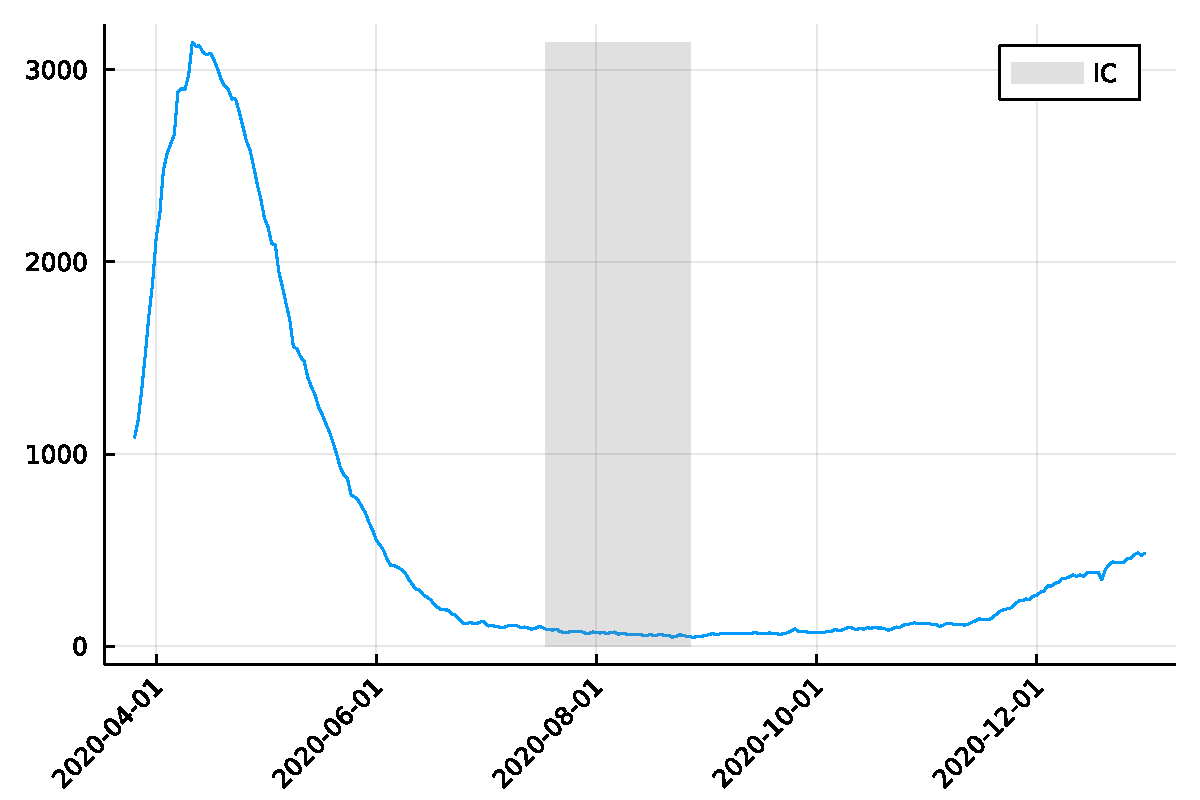
\includegraphics[width=\linewidth]{jl_64fcHC/admissionsICU_5_1.pdf}

We then isolate the IC and OC data. This code reproduces Figure ?? in the paper.


\begin{lstlisting}
(*@\HLJLn{y}@*) (*@\HLJLoB{=}@*) (*@\HLJLn{y2020}@*)(*@\HLJLp{[[}@*)(*@\HLJLn{ic{\_}2020}@*)(*@\HLJLp{;}@*) (*@\HLJLn{oc{\_}2020}@*)(*@\HLJLp{]]}@*)
(*@\HLJLn{days}@*) (*@\HLJLoB{=}@*) (*@\HLJLn{days2020}@*)(*@\HLJLp{[[}@*)(*@\HLJLn{ic{\_}2020}@*)(*@\HLJLp{;}@*) (*@\HLJLn{oc{\_}2020}@*)(*@\HLJLp{]]}@*)

(*@\HLJLn{ic{\_}idx}@*) (*@\HLJLoB{=}@*) (*@\HLJLni{1}@*)(*@\HLJLoB{:}@*)(*@\HLJLn{n{\_}ic}@*)
(*@\HLJLn{oc{\_}idx}@*) (*@\HLJLoB{=}@*) (*@\HLJLp{(}@*)(*@\HLJLn{n{\_}ic}@*)(*@\HLJLoB{+}@*)(*@\HLJLni{1}@*)(*@\HLJLp{)}@*)(*@\HLJLoB{:}@*)(*@\HLJLp{(}@*)(*@\HLJLn{n{\_}ic}@*)(*@\HLJLoB{+}@*)(*@\HLJLn{n{\_}oc}@*)(*@\HLJLp{)}@*)
(*@\HLJLn{yIC}@*) (*@\HLJLoB{=}@*) (*@\HLJLn{y}@*)(*@\HLJLp{[}@*)(*@\HLJLn{ic{\_}idx}@*)(*@\HLJLp{]}@*)
(*@\HLJLn{daysIC}@*) (*@\HLJLoB{=}@*) (*@\HLJLn{days}@*)(*@\HLJLp{[}@*)(*@\HLJLn{ic{\_}idx}@*)(*@\HLJLp{]}@*)
(*@\HLJLn{yOC}@*) (*@\HLJLoB{=}@*) (*@\HLJLn{y}@*)(*@\HLJLp{[}@*)(*@\HLJLn{oc{\_}idx}@*)(*@\HLJLp{]}@*)
(*@\HLJLn{daysOC}@*) (*@\HLJLoB{=}@*) (*@\HLJLn{days}@*)(*@\HLJLp{[}@*)(*@\HLJLn{oc{\_}idx}@*)(*@\HLJLp{]}@*)

(*@\HLJLnf{println}@*)(*@\HLJLp{(}@*)(*@\HLJLs{"{}In-control}@*) (*@\HLJLs{data:}@*) (*@\HLJLs{"{}}@*)(*@\HLJLp{,}@*) (*@\HLJLn{daysIC}@*)(*@\HLJLp{[[}@*)(*@\HLJLni{1}@*)(*@\HLJLp{,}@*) (*@\HLJLk{end}@*)(*@\HLJLp{]])}@*)
(*@\HLJLn{pl}@*) (*@\HLJLoB{=}@*) (*@\HLJLnf{plot}@*)(*@\HLJLp{(}@*)(*@\HLJLn{days}@*)(*@\HLJLp{,}@*) (*@\HLJLn{y}@*)(*@\HLJLp{,}@*) (*@\HLJLn{label}@*)(*@\HLJLoB{=}@*)(*@\HLJLs{"{}"{}}@*)(*@\HLJLp{,}@*) (*@\HLJLn{dpi}@*)(*@\HLJLoB{=}@*)(*@\HLJLni{400}@*)(*@\HLJLp{,}@*) (*@\HLJLn{xrotation}@*)(*@\HLJLoB{=}@*)(*@\HLJLni{45}@*)(*@\HLJLp{,}@*) (*@\HLJLn{bottom{\_}margin}@*)(*@\HLJLoB{=}@*)(*@\HLJLni{3}@*)(*@\HLJLn{mm}@*)(*@\HLJLp{)}@*)
(*@\HLJLnf{plot!}@*)(*@\HLJLp{(}@*)(*@\HLJLn{pl}@*)(*@\HLJLp{,}@*) (*@\HLJLn{days}@*)(*@\HLJLp{[}@*)(*@\HLJLni{1}@*)(*@\HLJLoB{:}@*)(*@\HLJLn{n{\_}ic}@*)(*@\HLJLp{],}@*) (*@\HLJLnf{fill}@*)(*@\HLJLp{(}@*)(*@\HLJLni{0}@*)(*@\HLJLp{,}@*) (*@\HLJLn{n{\_}ic}@*)(*@\HLJLp{),}@*) (*@\HLJLn{fillrange}@*)(*@\HLJLoB{=}@*)(*@\HLJLnf{fill}@*)(*@\HLJLp{(}@*)(*@\HLJLnf{maximum}@*)(*@\HLJLp{(}@*)(*@\HLJLn{y}@*)(*@\HLJLp{),}@*) (*@\HLJLn{n{\_}ic}@*)(*@\HLJLp{),}@*) (*@\HLJLn{color}@*)(*@\HLJLoB{=:}@*)(*@\HLJLn{gray}@*)(*@\HLJLp{,}@*) (*@\HLJLn{fillcolor}@*) (*@\HLJLoB{=}@*) (*@\HLJLs{"{}gray"{}}@*)(*@\HLJLp{,}@*) (*@\HLJLn{fillalpha}@*)(*@\HLJLoB{=}@*)(*@\HLJLnfB{0.25}@*)(*@\HLJLp{,}@*) (*@\HLJLn{alpha}@*)(*@\HLJLoB{=}@*)(*@\HLJLnfB{0.0}@*)(*@\HLJLp{,}@*) (*@\HLJLn{label}@*)(*@\HLJLoB{=}@*)(*@\HLJLs{"{}IC"{}}@*)(*@\HLJLp{,}@*) (*@\HLJLn{legend}@*)(*@\HLJLoB{=:}@*)(*@\HLJLn{bottomright}@*)(*@\HLJLp{)}@*)
(*@\HLJLn{\ensuremath{\tau}}@*) (*@\HLJLoB{=}@*) (*@\HLJLn{n{\_}ic}@*) (*@\HLJLoB{+}@*) (*@\HLJLni{29}@*)
(*@\HLJLnf{vline!}@*)(*@\HLJLp{([}@*)(*@\HLJLn{days}@*)(*@\HLJLp{[}@*)(*@\HLJLn{\ensuremath{\tau}}@*)(*@\HLJLp{]],}@*) (*@\HLJLn{color}@*)(*@\HLJLoB{=:}@*)(*@\HLJLn{gray}@*)(*@\HLJLp{,}@*) (*@\HLJLn{linestyle}@*)(*@\HLJLoB{=:}@*)(*@\HLJLn{dot}@*)(*@\HLJLp{,}@*) (*@\HLJLn{linewidth}@*)(*@\HLJLoB{=}@*)(*@\HLJLni{2}@*)(*@\HLJLp{,}@*)  (*@\HLJLn{label}@*)(*@\HLJLoB{=}@*)(*@\HLJLs{"{}"{}}@*)(*@\HLJLp{,}@*) (*@\HLJLn{markersize}@*)(*@\HLJLoB{=}@*)(*@\HLJLnfB{2.5}@*)(*@\HLJLp{)}@*)
(*@\HLJLnf{display}@*)(*@\HLJLp{(}@*)(*@\HLJLn{pl}@*)(*@\HLJLp{)}@*)
(*@\HLJLcs{{\#}}@*) (*@\HLJLcs{safesave(plotsdir(fold,}@*) (*@\HLJLcs{"{}ICU-IC-OC.png"{}),}@*) (*@\HLJLcs{pl)}@*)

(*@\HLJLnf{println}@*)(*@\HLJLp{(}@*)(*@\HLJLs{"{}Possible}@*) (*@\HLJLs{change-point}@*) (*@\HLJLs{location:}@*) (*@\HLJLs{"{}}@*)(*@\HLJLp{,}@*) (*@\HLJLn{days}@*)(*@\HLJLp{[}@*)(*@\HLJLn{\ensuremath{\tau}}@*)(*@\HLJLp{])}@*)
\end{lstlisting}

\begin{lstlisting}
In-control data: [Dates.Date((*@{"{}}@*)2020-07-18(*@{"{}}@*)), Dates.Date((*@{"{}}@*)2020-08-27(*@{"{}}@*))]
Possible change-point location: 2020-09-25
\end{lstlisting}

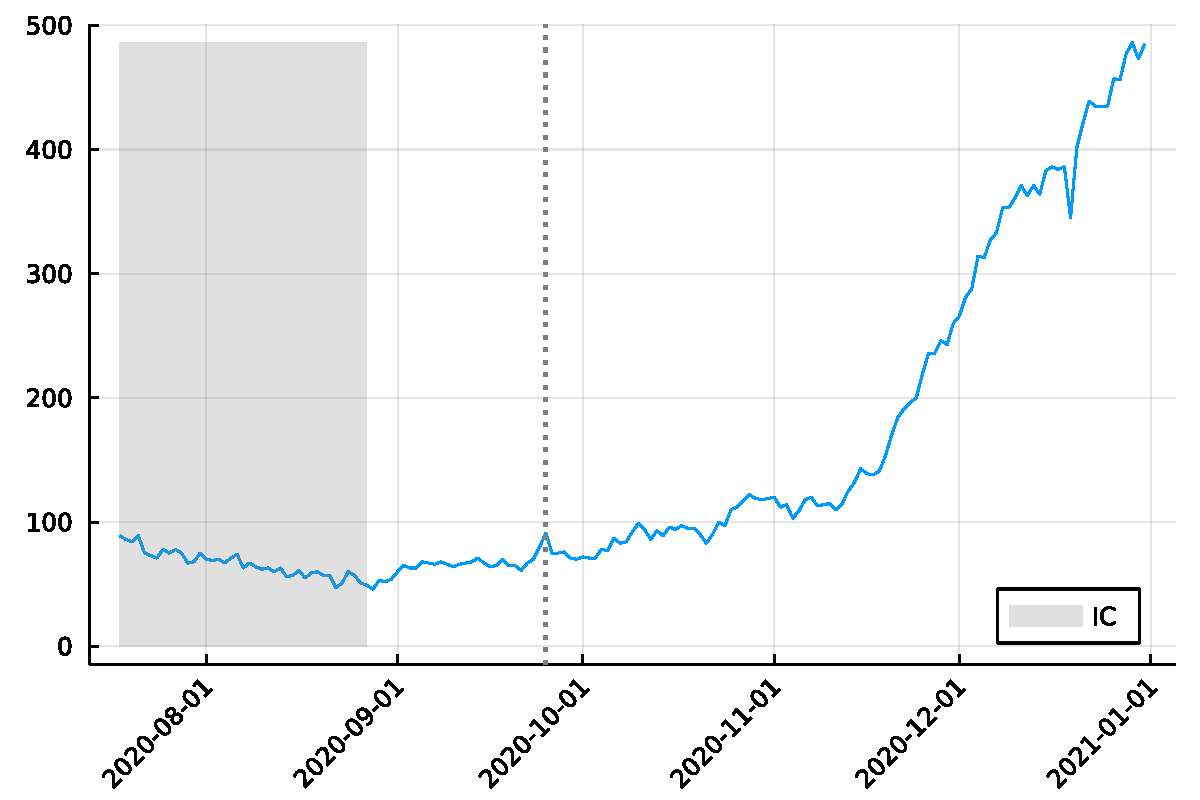
\includegraphics[width=\linewidth]{jl_64fcHC/admissionsICU_6_1.pdf}

We then calculate the initial estimate $\hat{\theta}$ and set the nominal IC ARL alongside the GICP probability $\beta$.


\begin{lstlisting}
(*@\HLJLn{thetaHat}@*) (*@\HLJLoB{=}@*) (*@\HLJLnf{mean}@*)(*@\HLJLp{(}@*)(*@\HLJLn{yIC}@*)(*@\HLJLp{)}@*)
(*@\HLJLn{Arl0}@*) (*@\HLJLoB{=}@*) (*@\HLJLni{500}@*)
(*@\HLJLn{beta}@*) (*@\HLJLoB{=}@*) (*@\HLJLnfB{0.05}@*)
\end{lstlisting}

\begin{lstlisting}
0.05
\end{lstlisting}


Next, we define a function that implements the control chart procedures using the various update mechanisms (AE, FE, CLM) that are defined in the source code.


\begin{lstlisting}
(*@\HLJLk{function}@*) (*@\HLJLnf{applyChart}@*)(*@\HLJLp{(}@*)(*@\HLJLn{ch}@*)(*@\HLJLp{,}@*) (*@\HLJLn{um}@*)(*@\HLJLp{,}@*) (*@\HLJLn{thetaHat}@*)(*@\HLJLp{,}@*) (*@\HLJLn{m}@*)(*@\HLJLp{,}@*) (*@\HLJLn{yprosp}@*)(*@\HLJLp{;}@*) (*@\HLJLn{seed}@*) (*@\HLJLoB{=}@*) (*@\HLJLni{123}@*)(*@\HLJLp{)}@*)
    (*@\HLJLcs{{\#}}@*) (*@\HLJLcs{Random.seed!(seed)}@*)
    (*@\HLJLn{maxrl{\_}i}@*) (*@\HLJLoB{=}@*) (*@\HLJLnf{length}@*)(*@\HLJLp{(}@*)(*@\HLJLn{yprosp}@*)(*@\HLJLp{)}@*)
    (*@\HLJLn{thetaHatVec}@*) (*@\HLJLoB{=}@*) (*@\HLJLnf{zeros}@*)(*@\HLJLp{(}@*)(*@\HLJLn{maxrl{\_}i}@*)(*@\HLJLp{)}@*)
    (*@\HLJLn{thetaHatVec}@*)(*@\HLJLp{[}@*)(*@\HLJLni{1}@*)(*@\HLJLp{]}@*) (*@\HLJLoB{=}@*) (*@\HLJLn{thetaHat}@*)
    (*@\HLJLn{di}@*) (*@\HLJLoB{=}@*) (*@\HLJLni{1}@*)
    (*@\HLJLn{diVec}@*) (*@\HLJLoB{=}@*) (*@\HLJLnf{Array}@*)(*@\HLJLp{{\{}}@*)(*@\HLJLn{Int}@*)(*@\HLJLp{{\}}(}@*)(*@\HLJLn{undef}@*)(*@\HLJLp{,}@*) (*@\HLJLn{maxrl{\_}i}@*)(*@\HLJLp{)}@*)
    (*@\HLJLn{diVec}@*)(*@\HLJLp{[}@*)(*@\HLJLni{1}@*)(*@\HLJLp{]}@*) (*@\HLJLoB{=}@*) (*@\HLJLn{di}@*)
    (*@\HLJLn{thetaHatCaut}@*) (*@\HLJLoB{=}@*) (*@\HLJLn{thetaHat}@*)
    (*@\HLJLn{thetaHatCautVec}@*) (*@\HLJLoB{=}@*) (*@\HLJLnf{zeros}@*)(*@\HLJLp{(}@*)(*@\HLJLn{maxrl{\_}i}@*)(*@\HLJLp{)}@*)
    (*@\HLJLn{thetaHatCautVec}@*)(*@\HLJLp{[}@*)(*@\HLJLni{1}@*)(*@\HLJLp{]}@*) (*@\HLJLoB{=}@*) (*@\HLJLn{thetaHatCaut}@*)

    (*@\HLJLn{t{\_}alarm}@*) (*@\HLJLoB{=}@*) (*@\HLJLnf{zeros}@*)(*@\HLJLp{(}@*)(*@\HLJLni{0}@*)(*@\HLJLp{)}@*)

    (*@\HLJLn{valueVec}@*) (*@\HLJLoB{=}@*) (*@\HLJLnf{zeros}@*)(*@\HLJLp{(}@*)(*@\HLJLn{maxrl{\_}i}@*)(*@\HLJLp{)}@*)
    (*@\HLJLn{valueVec}@*)(*@\HLJLp{[}@*)(*@\HLJLni{1}@*)(*@\HLJLp{]}@*) (*@\HLJLoB{=}@*) (*@\HLJLnf{get{\_}value}@*)(*@\HLJLp{(}@*)(*@\HLJLn{ch}@*)(*@\HLJLp{)}@*)
    (*@\HLJLn{i}@*) (*@\HLJLoB{=}@*) (*@\HLJLni{1}@*)
    (*@\HLJLk{while}@*) (*@\HLJLn{i}@*) (*@\HLJLoB{<}@*) (*@\HLJLn{maxrl{\_}i}@*)
        (*@\HLJLn{thetaHatCaut}@*) (*@\HLJLoB{=}@*) (*@\HLJLn{thetaHatVec}@*)(*@\HLJLp{[}@*)(*@\HLJLn{i}@*) (*@\HLJLoB{-}@*) (*@\HLJLn{di}@*) (*@\HLJLoB{+}@*) (*@\HLJLni{1}@*)(*@\HLJLp{]}@*)
        (*@\HLJLn{y}@*) (*@\HLJLoB{=}@*) (*@\HLJLn{yprosp}@*)(*@\HLJLp{[}@*)(*@\HLJLn{i}@*)(*@\HLJLp{]}@*)
        (*@\HLJLn{ch}@*) (*@\HLJLoB{=}@*) (*@\HLJLnf{update{\_}series}@*)(*@\HLJLp{(}@*)(*@\HLJLn{ch}@*)(*@\HLJLp{,}@*) (*@\HLJLnf{chart{\_}statistic}@*)(*@\HLJLp{(}@*)(*@\HLJLn{y}@*)(*@\HLJLp{,}@*) (*@\HLJLn{thetaHatCaut}@*)(*@\HLJLp{))}@*)
        (*@\HLJLn{thetaHat}@*) (*@\HLJLoB{=}@*) (*@\HLJLnf{update{\_}parameter}@*)(*@\HLJLp{(}@*)(*@\HLJLn{thetaHat}@*)(*@\HLJLp{,}@*) (*@\HLJLn{y}@*)(*@\HLJLp{,}@*) (*@\HLJLn{i}@*) (*@\HLJLoB{+}@*) (*@\HLJLn{m}@*)(*@\HLJLp{)}@*)
        (*@\HLJLn{i}@*) (*@\HLJLoB{+=}@*) (*@\HLJLni{1}@*)
        (*@\HLJLn{valueVec}@*)(*@\HLJLp{[}@*)(*@\HLJLn{i}@*)(*@\HLJLp{]}@*) (*@\HLJLoB{=}@*) (*@\HLJLnf{get{\_}value}@*)(*@\HLJLp{(}@*)(*@\HLJLn{ch}@*)(*@\HLJLp{)}@*)
        (*@\HLJLn{thetaHatVec}@*)(*@\HLJLp{[}@*)(*@\HLJLn{i}@*)(*@\HLJLp{]}@*) (*@\HLJLoB{=}@*) (*@\HLJLn{thetaHat}@*)
        (*@\HLJLk{if}@*) (*@\HLJLnf{check{\_}update}@*)(*@\HLJLp{(}@*)(*@\HLJLn{ch}@*)(*@\HLJLp{,}@*) (*@\HLJLn{um}@*)(*@\HLJLp{)}@*)
            (*@\HLJLn{di}@*) (*@\HLJLoB{=}@*) (*@\HLJLni{1}@*)
        (*@\HLJLk{else}@*)
            (*@\HLJLn{di}@*) (*@\HLJLoB{+=}@*) (*@\HLJLni{1}@*)
        (*@\HLJLk{end}@*)
        (*@\HLJLn{diVec}@*)(*@\HLJLp{[}@*)(*@\HLJLn{i}@*)(*@\HLJLp{]}@*) (*@\HLJLoB{=}@*) (*@\HLJLn{di}@*)
        (*@\HLJLn{thetaHatCautVec}@*)(*@\HLJLp{[}@*)(*@\HLJLn{i}@*)(*@\HLJLp{]}@*) (*@\HLJLoB{=}@*) (*@\HLJLn{thetaHatCaut}@*)
        (*@\HLJLk{if}@*) (*@\HLJLnf{check{\_}OC}@*)(*@\HLJLp{(}@*)(*@\HLJLn{ch}@*)(*@\HLJLp{)}@*)
            (*@\HLJLnf{push!}@*)(*@\HLJLp{(}@*)(*@\HLJLn{t{\_}alarm}@*)(*@\HLJLp{,}@*) (*@\HLJLn{i}@*)(*@\HLJLp{)}@*)
        (*@\HLJLk{end}@*)
    (*@\HLJLk{end}@*)

    (*@\HLJLk{return}@*) (*@\HLJLp{(}@*)(*@\HLJLn{t{\_}alarm}@*) (*@\HLJLoB{=}@*) (*@\HLJLn{t{\_}alarm}@*)(*@\HLJLp{,}@*) (*@\HLJLn{dat}@*) (*@\HLJLoB{=}@*) (*@\HLJLn{yprosp}@*)(*@\HLJLp{,}@*) (*@\HLJLn{chart{\_}values}@*) (*@\HLJLoB{=}@*) (*@\HLJLn{valueVec}@*)(*@\HLJLp{,}@*) (*@\HLJLn{limit{\_}alarm}@*) (*@\HLJLoB{=}@*) (*@\HLJLnf{get{\_}limits}@*)(*@\HLJLp{(}@*)(*@\HLJLn{ch}@*)(*@\HLJLp{),}@*) (*@\HLJLn{limit{\_}cautious}@*) (*@\HLJLoB{=}@*) (*@\HLJLnf{get{\_}warning{\_}limit}@*)(*@\HLJLp{(}@*)(*@\HLJLn{um}@*)(*@\HLJLp{),}@*) (*@\HLJLn{parameter{\_}updates}@*) (*@\HLJLoB{=}@*) (*@\HLJLn{thetaHatCautVec}@*)(*@\HLJLp{,}@*) (*@\HLJLn{di}@*) (*@\HLJLoB{=}@*) (*@\HLJLn{diVec}@*)(*@\HLJLp{)}@*)
(*@\HLJLk{end}@*)
\end{lstlisting}

\begin{lstlisting}
applyChart (generic function with 1 method)
\end{lstlisting}


Furthermore, we define a function that applies the control chart to a prospective monitoring data after having corrected the control limit to satisfy the GICP condition.


\begin{lstlisting}
(*@\HLJLk{function}@*) (*@\HLJLnf{applyChartGICP}@*)(*@\HLJLp{(}@*)(*@\HLJLn{ch}@*)(*@\HLJLp{,}@*) (*@\HLJLn{um}@*)(*@\HLJLp{,}@*) (*@\HLJLn{yinit}@*)(*@\HLJLp{,}@*) (*@\HLJLn{yprosp}@*)(*@\HLJLp{,}@*) (*@\HLJLn{thetaHat}@*)(*@\HLJLp{,}@*) (*@\HLJLn{Arl0}@*)(*@\HLJLp{;}@*) (*@\HLJLn{beta}@*)(*@\HLJLoB{::}@*)(*@\HLJLnf{Union}@*)(*@\HLJLp{{\{}}@*)(*@\HLJLn{Bool}@*)(*@\HLJLp{,}@*) (*@\HLJLn{Float64}@*)(*@\HLJLp{{\}}}@*) (*@\HLJLoB{=}@*) (*@\HLJLnfB{0.2}@*)(*@\HLJLp{,}@*) (*@\HLJLn{maxrl}@*)(*@\HLJLoB{=}@*)(*@\HLJLnfB{1e04}@*)(*@\HLJLp{,}@*) (*@\HLJLn{verbose}@*)(*@\HLJLoB{=}@*)(*@\HLJLkc{true}@*)(*@\HLJLp{,}@*) (*@\HLJLn{seed}@*)(*@\HLJLoB{=}@*)(*@\HLJLnf{Int}@*)(*@\HLJLp{(}@*)(*@\HLJLnf{rand}@*)(*@\HLJLp{(}@*)(*@\HLJLni{1}@*)(*@\HLJLoB{:}@*)(*@\HLJLnfB{1e06}@*)(*@\HLJLp{)))}@*)
    (*@\HLJLn{m}@*) (*@\HLJLoB{=}@*) (*@\HLJLnf{length}@*)(*@\HLJLp{(}@*)(*@\HLJLn{yinit}@*)(*@\HLJLp{)}@*)
    (*@\HLJLk{if}@*) (*@\HLJLnf{isa}@*)(*@\HLJLp{(}@*)(*@\HLJLn{um}@*)(*@\HLJLp{,}@*) (*@\HLJLn{CautiousLearning}@*)(*@\HLJLp{)}@*)
        (*@\HLJLn{Ats0}@*) (*@\HLJLoB{=}@*) (*@\HLJLnf{get{\_}ATS}@*)(*@\HLJLp{(}@*)(*@\HLJLn{um}@*)(*@\HLJLp{)}@*)
        (*@\HLJLk{if}@*) (*@\HLJLn{Ats0}@*) (*@\HLJLoB{!=}@*) (*@\HLJLni{0}@*)
            (*@\HLJLcs{{\#}}@*) (*@\HLJLcs{Calculate}@*) (*@\HLJLcs{limit}@*) (*@\HLJLcs{if}@*) (*@\HLJLcs{Ats0}@*) (*@\HLJLcs{!=}@*) (*@\HLJLcs{0,}@*) (*@\HLJLcs{otherwise}@*) (*@\HLJLcs{use}@*) (*@\HLJLcs{zero-restarting}@*) (*@\HLJLcs{chart}@*)
            (*@\HLJLk{if}@*) (*@\HLJLn{verbose}@*) (*@\HLJLnf{println}@*)(*@\HLJLp{(}@*)(*@\HLJLs{"{}Calculating}@*) (*@\HLJLs{limits}@*) (*@\HLJLs{for}@*) (*@\HLJLs{target}@*) (*@\HLJLs{ATS..."{}}@*)(*@\HLJLp{)}@*) (*@\HLJLk{end}@*)
            (*@\HLJLn{sa{\_}ats}@*) (*@\HLJLoB{=}@*) (*@\HLJLnf{saControlLimits}@*)(*@\HLJLp{(}@*)(*@\HLJLn{ch}@*)(*@\HLJLp{,}@*) (*@\HLJLnf{AdaptiveEstimator}@*)(*@\HLJLp{(),}@*) (*@\HLJLn{runSimulation}@*)(*@\HLJLp{,}@*) (*@\HLJLn{Ats0}@*)(*@\HLJLp{,}@*) (*@\HLJLn{thetaHat}@*)(*@\HLJLp{,}@*) (*@\HLJLnf{Poisson}@*)(*@\HLJLp{(}@*)(*@\HLJLn{thetaHat}@*)(*@\HLJLp{),}@*)
                                    (*@\HLJLn{m}@*)(*@\HLJLp{,}@*) (*@\HLJLn{verbose}@*)(*@\HLJLoB{=}@*)(*@\HLJLkc{false}@*)(*@\HLJLp{,}@*) (*@\HLJLn{Amin}@*)(*@\HLJLoB{=}@*)(*@\HLJLnfB{0.1}@*)(*@\HLJLp{,}@*) (*@\HLJLn{maxiter}@*)(*@\HLJLoB{=}@*)(*@\HLJLnfB{1e05}@*)(*@\HLJLp{,}@*)
                                    (*@\HLJLn{gamma}@*)(*@\HLJLoB{=}@*)(*@\HLJLnfB{0.015}@*)(*@\HLJLp{,}@*) (*@\HLJLn{adjusted}@*)(*@\HLJLoB{=}@*)(*@\HLJLkc{true}@*)(*@\HLJLp{,}@*) (*@\HLJLn{seed}@*)(*@\HLJLoB{=}@*)(*@\HLJLn{seed}@*)(*@\HLJLp{)}@*)
            (*@\HLJLn{um}@*) (*@\HLJLoB{=}@*) (*@\HLJLnf{CautiousLearning}@*)(*@\HLJLp{(}@*)(*@\HLJLn{L}@*) (*@\HLJLoB{=}@*) (*@\HLJLn{sa{\_}ats}@*)(*@\HLJLp{[}@*)(*@\HLJLsc{:h}@*)(*@\HLJLp{],}@*) (*@\HLJLn{ATS}@*) (*@\HLJLoB{=}@*) (*@\HLJLn{Ats0}@*)(*@\HLJLp{)}@*)
        (*@\HLJLk{else}@*)
            (*@\HLJLk{if}@*) (*@\HLJLn{verbose}@*) (*@\HLJLnf{println}@*)(*@\HLJLp{(}@*)(*@\HLJLs{"{}ATS}@*) (*@\HLJLs{=}@*) (*@\HLJLs{0,}@*) (*@\HLJLs{skipping}@*) (*@\HLJLs{limit}@*) (*@\HLJLs{calculation."{}}@*)(*@\HLJLp{)}@*) (*@\HLJLk{end}@*)
        (*@\HLJLk{end}@*)
        (*@\HLJLcs{{\#}}@*) (*@\HLJLcs{Estimate}@*) (*@\HLJLcs{cautious}@*) (*@\HLJLcs{learning}@*) (*@\HLJLcs{limit}@*)
    (*@\HLJLk{end}@*)

    (*@\HLJLk{if}@*) (*@\HLJLn{beta}@*) (*@\HLJLoB{==}@*) (*@\HLJLkc{false}@*)
        (*@\HLJLn{chart}@*) (*@\HLJLoB{=}@*) (*@\HLJLnf{deepcopy}@*)(*@\HLJLp{(}@*)(*@\HLJLn{ch}@*)(*@\HLJLp{)}@*)
    (*@\HLJLk{else}@*)
        (*@\HLJLn{chart}@*) (*@\HLJLoB{=}@*) (*@\HLJLnf{adjust{\_}chart{\_}gicp}@*)(*@\HLJLp{(}@*)(*@\HLJLn{ch}@*)(*@\HLJLp{,}@*) (*@\HLJLn{um}@*)(*@\HLJLp{,}@*) (*@\HLJLn{yinit}@*)(*@\HLJLp{,}@*) (*@\HLJLn{thetaHat}@*)(*@\HLJLp{,}@*) (*@\HLJLn{runSimulation}@*)(*@\HLJLp{,}@*) (*@\HLJLn{m}@*)(*@\HLJLp{,}@*) (*@\HLJLn{Arl0}@*)(*@\HLJLp{,}@*) (*@\HLJLn{beta}@*)(*@\HLJLoB{=}@*)(*@\HLJLn{beta}@*)(*@\HLJLp{,}@*) (*@\HLJLn{verbose}@*)(*@\HLJLoB{=}@*)(*@\HLJLn{verbose}@*)(*@\HLJLp{)}@*)
    (*@\HLJLk{end}@*)

    (*@\HLJLk{return}@*) (*@\HLJLnf{applyChart}@*)(*@\HLJLp{(}@*)(*@\HLJLn{chart}@*)(*@\HLJLp{,}@*) (*@\HLJLn{um}@*)(*@\HLJLp{,}@*) (*@\HLJLn{thetaHat}@*)(*@\HLJLp{,}@*) (*@\HLJLn{m}@*)(*@\HLJLp{,}@*) (*@\HLJLn{yprosp}@*)(*@\HLJLp{)}@*)
(*@\HLJLk{end}@*)
\end{lstlisting}

\begin{lstlisting}
applyChartGICP (generic function with 1 method)
\end{lstlisting}


The GICP control limit correction uses the \texttt{adjust\_chart\_gicp} function defined in the source code, which implements the computations described in Subsection ??.

We finally apply the control charts using the methods and obtain the results.  This code reproduces Figure ?? and Table ??.


\begin{lstlisting}
(*@\HLJLn{Random}@*)(*@\HLJLoB{.}@*)(*@\HLJLnf{seed!}@*)(*@\HLJLp{(}@*)(*@\HLJLni{2022}@*)(*@\HLJLoB{-}@*)(*@\HLJLni{08}@*)(*@\HLJLoB{-}@*)(*@\HLJLni{18}@*)(*@\HLJLp{)}@*)
(*@\HLJLn{D}@*) (*@\HLJLoB{=}@*) (*@\HLJLn{Poisson}@*)
(*@\HLJLn{fname}@*) (*@\HLJLoB{=}@*) (*@\HLJLnf{plotsdir}@*)(*@\HLJLp{(}@*)(*@\HLJLn{fold}@*)(*@\HLJLp{,}@*) (*@\HLJLs{"{}alarms.jld2"{}}@*)(*@\HLJLp{)}@*)

(*@\HLJLn{umVec}@*) (*@\HLJLoB{=}@*) (*@\HLJLp{[}@*)(*@\HLJLnf{CautiousLearning}@*)(*@\HLJLp{(}@*)(*@\HLJLn{ATS}@*)(*@\HLJLoB{=}@*)(*@\HLJLni{0}@*)(*@\HLJLp{),}@*) (*@\HLJLnf{FixedParameter}@*)(*@\HLJLp{(),}@*) (*@\HLJLnf{AdaptiveEstimator}@*)(*@\HLJLp{()]}@*)
(*@\HLJLn{nms}@*) (*@\HLJLoB{=}@*) (*@\HLJLp{[}@*)(*@\HLJLs{"{}CLM"{}}@*)(*@\HLJLp{,}@*) (*@\HLJLs{"{}FE"{}}@*)(*@\HLJLp{,}@*) (*@\HLJLs{"{}AE"{}}@*)(*@\HLJLp{]}@*)
(*@\HLJLn{perf}@*) (*@\HLJLoB{=}@*) (*@\HLJLp{[]}@*)
(*@\HLJLn{L}@*) (*@\HLJLoB{=}@*) (*@\HLJLp{[]}@*)
(*@\HLJLk{for}@*) (*@\HLJLn{i}@*) (*@\HLJLkp{in}@*) (*@\HLJLnf{eachindex}@*)(*@\HLJLp{(}@*)(*@\HLJLn{umVec}@*)(*@\HLJLp{)}@*)
    (*@\HLJLn{ch}@*) (*@\HLJLoB{=}@*) (*@\HLJLnf{signedEWMA}@*)(*@\HLJLp{(}@*)(*@\HLJLn{l}@*)(*@\HLJLoB{=}@*)(*@\HLJLnfB{0.2}@*)(*@\HLJLp{,}@*) (*@\HLJLn{L}@*) (*@\HLJLoB{=}@*) (*@\HLJLnfB{1.0}@*)(*@\HLJLp{)}@*)
    (*@\HLJLn{um}@*) (*@\HLJLoB{=}@*) (*@\HLJLn{umVec}@*)(*@\HLJLp{[}@*)(*@\HLJLn{i}@*)(*@\HLJLp{]}@*)
    (*@\HLJLn{res}@*) (*@\HLJLoB{=}@*) (*@\HLJLnf{applyChartGICP}@*)(*@\HLJLp{(}@*)(*@\HLJLn{ch}@*)(*@\HLJLp{,}@*) (*@\HLJLn{um}@*)(*@\HLJLp{,}@*) (*@\HLJLn{yIC}@*)(*@\HLJLp{,}@*) (*@\HLJLn{yOC}@*)(*@\HLJLp{,}@*) (*@\HLJLn{thetaHat}@*)(*@\HLJLp{,}@*) (*@\HLJLn{Arl0}@*)(*@\HLJLp{,}@*) (*@\HLJLn{beta}@*)(*@\HLJLoB{=}@*)(*@\HLJLn{beta}@*)(*@\HLJLp{)}@*)
    (*@\HLJLnf{append!}@*)(*@\HLJLp{(}@*)(*@\HLJLn{L}@*)(*@\HLJLp{,}@*) (*@\HLJLn{res}@*)(*@\HLJLp{[}@*)(*@\HLJLsc{:limit{\_}alarm}@*)(*@\HLJLp{])}@*)
    (*@\HLJLn{plotsave}@*) (*@\HLJLoB{=}@*) (*@\HLJLnf{plotsdir}@*)(*@\HLJLp{(}@*)(*@\HLJLn{fold}@*)(*@\HLJLp{,}@*) (*@\HLJLn{nms}@*)(*@\HLJLp{[}@*)(*@\HLJLn{i}@*)(*@\HLJLp{]}@*)(*@\HLJLoB{*}@*)(*@\HLJLs{"{}.png"{}}@*)(*@\HLJLp{)}@*)
    (*@\HLJLn{pl}@*) (*@\HLJLoB{=}@*) (*@\HLJLnf{plot}@*)(*@\HLJLp{(}@*)(*@\HLJLn{res}@*)(*@\HLJLoB{.}@*)(*@\HLJLn{chart{\_}values}@*)(*@\HLJLp{[}@*)(*@\HLJLni{1}@*)(*@\HLJLoB{:}@*)(*@\HLJLni{55}@*)(*@\HLJLp{],}@*) (*@\HLJLn{label}@*)(*@\HLJLoB{=}@*)(*@\HLJLso{L"{}C{\_}t"{}}@*)(*@\HLJLp{,}@*) (*@\HLJLn{legend}@*)(*@\HLJLoB{=:}@*)(*@\HLJLn{outerright}@*)(*@\HLJLp{,}@*) (*@\HLJLn{dpi}@*)(*@\HLJLoB{=}@*)(*@\HLJLni{400}@*)(*@\HLJLp{)}@*)
    (*@\HLJLnf{hline!}@*)(*@\HLJLp{([}@*)(*@\HLJLn{res}@*)(*@\HLJLoB{.}@*)(*@\HLJLn{limit{\_}alarm}@*)(*@\HLJLp{],}@*) (*@\HLJLn{style}@*)(*@\HLJLoB{=:}@*)(*@\HLJLn{dash}@*)(*@\HLJLp{,}@*) (*@\HLJLn{colour}@*)(*@\HLJLoB{=}@*)(*@\HLJLs{"{}red"{}}@*)(*@\HLJLp{,}@*) (*@\HLJLn{xlab}@*)(*@\HLJLoB{=}@*)(*@\HLJLso{L"{}t"{}}@*)(*@\HLJLp{,}@*) (*@\HLJLn{ylab}@*)(*@\HLJLoB{=}@*)(*@\HLJLso{L"{}C{\_}t"{}}@*)(*@\HLJLp{,}@*) (*@\HLJLn{label}@*)(*@\HLJLoB{=}@*)(*@\HLJLs{"{}"{}}@*)(*@\HLJLp{)}@*)
    (*@\HLJLn{tau}@*) (*@\HLJLoB{=}@*) (*@\HLJLnf{Int}@*)(*@\HLJLp{(}@*)(*@\HLJLnf{first}@*)(*@\HLJLp{(}@*)(*@\HLJLn{res}@*)(*@\HLJLoB{.}@*)(*@\HLJLn{t{\_}alarm}@*)(*@\HLJLp{))}@*)
    (*@\HLJLnf{scatter!}@*)(*@\HLJLp{([}@*)(*@\HLJLn{tau}@*)(*@\HLJLp{],}@*) (*@\HLJLp{[}@*)(*@\HLJLn{res}@*)(*@\HLJLoB{.}@*)(*@\HLJLn{chart{\_}values}@*)(*@\HLJLp{[}@*)(*@\HLJLn{tau}@*)(*@\HLJLp{]],}@*) (*@\HLJLn{colour}@*)(*@\HLJLoB{=}@*)(*@\HLJLs{"{}red"{}}@*)(*@\HLJLp{,}@*) (*@\HLJLn{label}@*)(*@\HLJLoB{=}@*)(*@\HLJLs{"{}"{}}@*)(*@\HLJLp{)}@*)
    (*@\HLJLnf{display}@*)(*@\HLJLp{(}@*)(*@\HLJLn{pl}@*)(*@\HLJLp{)}@*)
    (*@\HLJLnf{append!}@*)(*@\HLJLp{(}@*)(*@\HLJLn{perf}@*)(*@\HLJLp{,}@*) (*@\HLJLn{tau}@*)(*@\HLJLp{)}@*)
    (*@\HLJLnf{println}@*)(*@\HLJLp{(}@*)(*@\HLJLn{tau}@*)(*@\HLJLp{,}@*)(*@\HLJLs{"{}}@*)(*@\HLJLse{{\textbackslash}t}@*)(*@\HLJLs{"{}}@*)(*@\HLJLp{,}@*) (*@\HLJLn{daysOC}@*)(*@\HLJLp{[}@*)(*@\HLJLn{tau}@*)(*@\HLJLp{])}@*)
(*@\HLJLk{end}@*)

(*@\HLJLnd{@rput}@*) (*@\HLJLn{nms}@*)
(*@\HLJLnd{@rput}@*) (*@\HLJLn{perf}@*)
(*@\HLJLnd{@rput}@*) (*@\HLJLn{L}@*)

(*@\HLJLn{tab}@*) (*@\HLJLoB{=}@*) (*@\HLJLso{R"{}"{}"{}}@*)
(*@\HLJLso{library(knitr)}@*)
(*@\HLJLso{library(kableExtra)}@*)
(*@\HLJLso{df}@*) (*@\HLJLso{=}@*) (*@\HLJLso{cbind(nms,}@*) (*@\HLJLso{perf,}@*) (*@\HLJLso{L)}@*)
(*@\HLJLso{tex{\_}OC}@*) (*@\HLJLso{<-}@*) (*@\HLJLso{kable(df,}@*) (*@\HLJLso{format="{}latex"{},}@*) (*@\HLJLso{booktabs=TRUE,}@*) (*@\HLJLso{digits}@*) (*@\HLJLso{=}@*) (*@\HLJLso{2,}@*) (*@\HLJLso{row.names=FALSE,}@*) (*@\HLJLso{col.names=c("{}Estimator"{},}@*) (*@\HLJLso{"{}Alarm"{},}@*) (*@\HLJLso{"{}Limit"{}),}@*) (*@\HLJLso{escape=FALSE,}@*) (*@\HLJLso{align={\textquotesingle}c{\textquotesingle},}@*) (*@\HLJLso{linesep}@*) (*@\HLJLso{=}@*) (*@\HLJLso{"{}"{},}@*)
    (*@\HLJLso{caption}@*) (*@\HLJLso{=}@*) (*@\HLJLso{"{}Time}@*) (*@\HLJLso{to}@*) (*@\HLJLso{alarm}@*) (*@\HLJLso{of}@*) (*@\HLJLso{the}@*) (*@\HLJLso{one-sided}@*) (*@\HLJLso{EWMA}@*) (*@\HLJLso{control}@*) (*@\HLJLso{chart}@*) (*@\HLJLso{using}@*) (*@\HLJLso{the}@*) (*@\HLJLso{fixed}@*) (*@\HLJLso{(FE),}@*) (*@\HLJLso{adaptive}@*) (*@\HLJLso{(AE)}@*) (*@\HLJLso{and}@*) (*@\HLJLso{the}@*) (*@\HLJLso{proposed}@*) (*@\HLJLso{cautious}@*) (*@\HLJLso{learning}@*) (*@\HLJLso{(CLM)}@*) (*@\HLJLso{update}@*) (*@\HLJLso{rules."{},}@*) (*@\HLJLso{label="{}ICU}@*) (*@\HLJLso{OC}@*) (*@\HLJLso{alarm"{})}@*) (*@\HLJLso{{\%}>{\%}}@*)
    (*@\HLJLso{kable{\_}styling(latex{\_}options}@*) (*@\HLJLso{=}@*) (*@\HLJLso{"{}HOLD{\_}position"{})}@*)
(*@\HLJLso{"{}"{}"{}}@*) (*@\HLJLoB{|>}@*) (*@\HLJLn{rcopy}@*)

(*@\HLJLnf{println}@*)(*@\HLJLp{(}@*)(*@\HLJLn{tab}@*)(*@\HLJLp{)}@*)
\end{lstlisting}

\begin{lstlisting}
ATS = 0, skipping limit calculation.
Calculating GICP for extremum 1/1...
GICP done.
30	2020-09-26
Calculating GICP for extremum 1/1...
GICP done.
41	2020-10-07
Calculating GICP for extremum 1/1...
GICP done.
31	2020-09-27
(*@{{\textbackslash}}@*)begin(*@{{\{}}@*)table(*@{{\}}}@*)[H]

(*@{{\textbackslash}}@*)caption(*@{{\{}}@*)(*@{{\textbackslash}}@*)label(*@{{\{}}@*)tab:ICU OC alarm(*@{{\}}}@*)Time to alarm of the one-sided EWMA contro
l chart using the fixed (FE), adaptive (AE) and the proposed cautious learn
ing (CLM) update rules.(*@{{\}}}@*)
(*@{{\textbackslash}}@*)centering
(*@{{\textbackslash}}@*)begin(*@{{\{}}@*)tabular(*@{{\}}}@*)[t](*@{{\{}}@*)ccc(*@{{\}}}@*)
(*@{{\textbackslash}}@*)toprule
Estimator (*@{{\&}}@*) Alarm (*@{{\&}}@*) Limit(*@{{\textbackslash}}@*)(*@{{\textbackslash}}@*)
(*@{{\textbackslash}}@*)midrule
CLM (*@{{\&}}@*) 30 (*@{{\&}}@*) 1.05469060798468(*@{{\textbackslash}}@*)(*@{{\textbackslash}}@*)
FE (*@{{\&}}@*) 41 (*@{{\&}}@*) 1.2147825075143(*@{{\textbackslash}}@*)(*@{{\textbackslash}}@*)
AE (*@{{\&}}@*) 31 (*@{{\&}}@*) 1.02214273823991(*@{{\textbackslash}}@*)(*@{{\textbackslash}}@*)
(*@{{\textbackslash}}@*)bottomrule
(*@{{\textbackslash}}@*)end(*@{{\{}}@*)tabular(*@{{\}}}@*)
(*@{{\textbackslash}}@*)end(*@{{\{}}@*)table(*@{{\}}}@*)
\end{lstlisting}

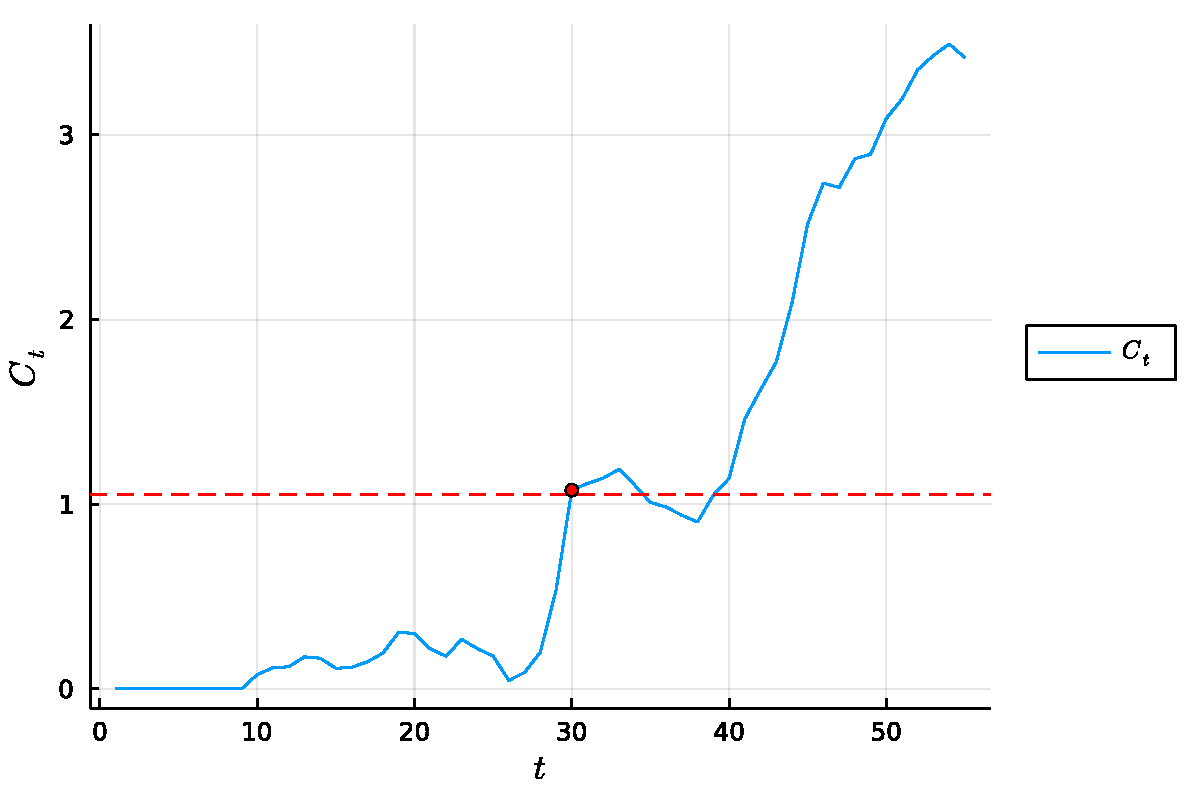
\includegraphics[width=\linewidth]{jl_64fcHC/admissionsICU_10_1.pdf}
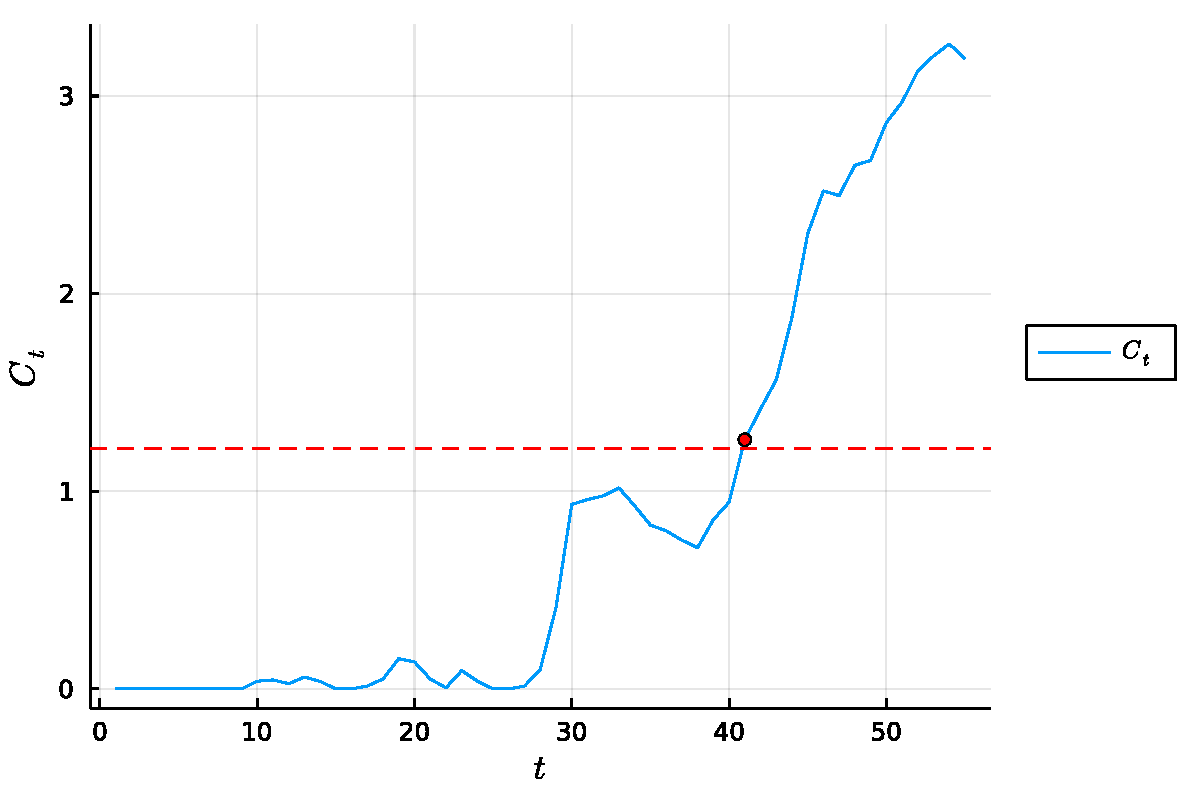
\includegraphics[width=\linewidth]{jl_64fcHC/admissionsICU_10_2.pdf}
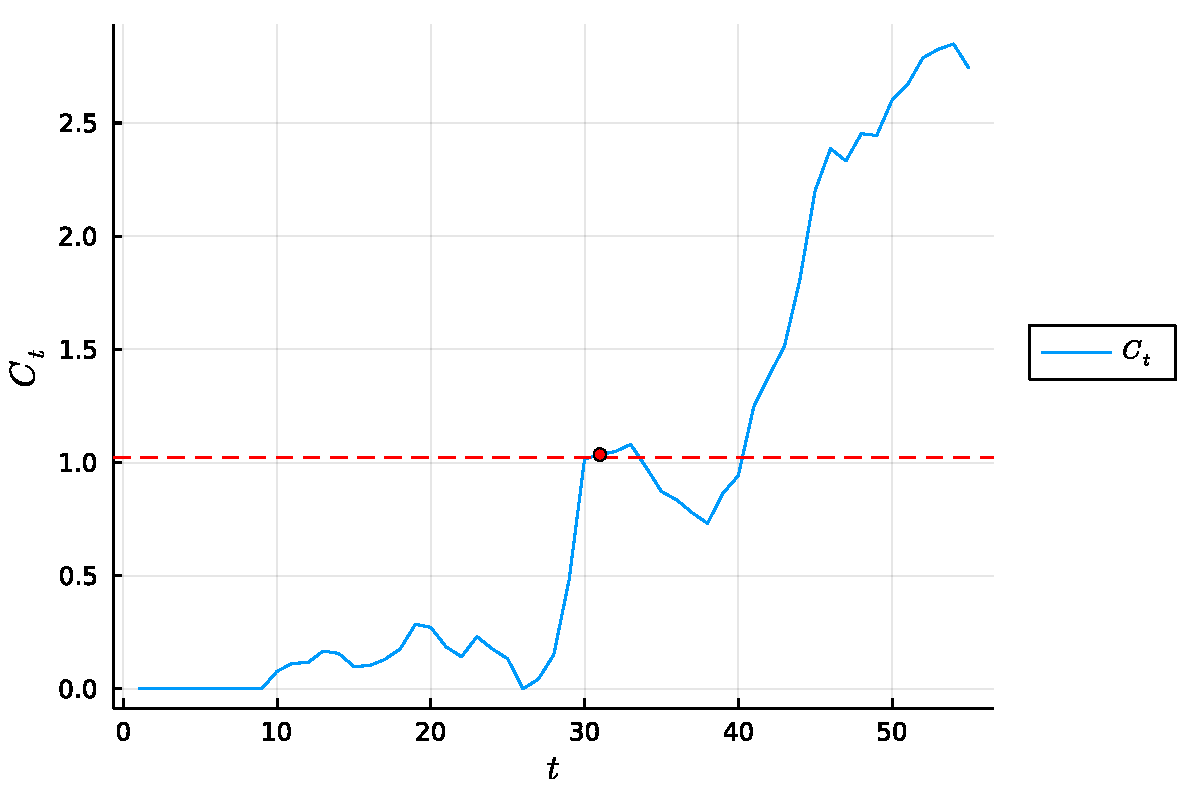
\includegraphics[width=\linewidth]{jl_64fcHC/admissionsICU_10_3.pdf}


\end{document}
